%In welchen Fachgegenst�nden kann Python noch verwendet werden? Vorstellen von m�glichen Einsatzgebieten in der Mathematik oder im Embedded Systems Bereich. 
	%Nicht-Fokus: Auflistung aller M�glichkeiten.
	%Fokus: Auswahl von 2-3 m�glichen Fachbereichen und kurzes Vorstellen dieser. F�r Details wird auf Literatur verwiesen.
	%Embedded Systems (siehe C Standard in Python History)
	
Wie aus den vorangegangenen Kapiteln hervorgeht, eignet sich Python hervorragend f�r den Einsatz im Informatikunterricht. Einerseits ist Python eine optimale Sprache, um das Programmieren zu lehren, andererseits k�nnen die grundlegenden Konzepte wie Programmierparadigmen und Algorithmen gut erarbeitet werden. 
	
In welchen Fachgegenst�nden kann Python noch verwendet werden? Und warum ist es gut, einen Unterrichtsgegestand mit Python zu unterst�tzen?
	
%\subsubsection*{Mathematik}
Diese Fragen sollen an einem Beispiel aus der \textbf{Mathematik} erl�utert werden.

\begin{lstlisting}[style=interpreter]
>>> def dreieckszahl(n):  return n*(n+1)/2
...
>>> [dreieckszahl(n) for n in range(1,10)]
[1, 3, 6, 10, 15, 21, 28, 36, 45]
\end{lstlisting}

\begin{figure}[h]
	\centering
	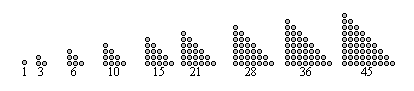
\includegraphics[scale=1]{graphics/dreieckszahl.png}
	\caption{Dreieckszahl}
	\label{fig:dreieckszahl}
\end{figure}

\cite{python:math} bedient sich des Beispiels der Dreieckszahl (Abbildung \ref{fig:dreieckszahl}) und meint, dass der Mathematikunterricht der perfekte Einstieg in das Programmieren ist. 

\begin{quote}
{\itshape "'What I like [...] is the connection between rule-driven (program driven) number sequences, such as 1, 3, 6, 10.. and the corresponding, visually appealing shapes. This forges connections between algebra and visualizations, but in a way more basic than by means of Cartesian coordinates (or any coordinates). Moreover such sequences provide an ideal beginning for learning to program..."'}
\end{quote}

Weiters geht daraus hervor, dass die Verkn�fung von Theorie, praktischer Umsetzung und dem visuellem Feedback durch den Interpreter, oder eine grafische Implementierung\footnote{z.B. mit VPython: http://vpython.org/} den Lernerfolg erh�hen kann.

Diese Aussage wird von \cite{python:broch} gest�tzt, wo es hei�t, dass der h�chste Lernerfolg durch \emph{aktive Lehrmethoden} und \emph{direkt gesteuerte Erfahrung} erzielt wird. Eine aktive Lehrmethode ist z.B. die Erarbeitung und Veranschaulichung der gelehrten Inhalte mittels Python.

%Damit ist die zweite Frage der Einleitung dieses Kapitels beantwortet. Um auch die Erste zu beantworten nennt der Autor noch..

Auch andere Themengebiete der Mathematik lassen sich gut mittels Python unterst�tzen. Induktion, Rekursion, Algebra, Vektoren, Funktionen, Wahrscheinlichkeit und Kryptographie\footnote{Python Cryptography Toolkit: http://www.amk.ca/python/code/crypto} sind nur Ausschnitte m�glicher Teilgebiete.

Folgend nun ein Auszug von Fachgegenst�nden, welche mit Python als unterst�tzendes Werkzeug bereichert werden k�nnen.

\begin{itemize}
	\item \textbf{Betriebssysteme} Prozesse, Threads, Semaphore, Queues, Stacks, ...
	\item \textbf{Internettechnologien} Client-Server Entwicklung, Protokolle, ...
	\item \textbf{Genetik}\footnote{pgapy: http://pgapy.sourceforge.net/ oder Biopython: http://biopython.org/} 
	%\item \textbf{Physik}?? Vpython ist aber schon als Fu�note erw�hnt, einstweilen ausgeblendet
	\item \textbf{3D Engineering}\footnote{Blender: http://www.blender.org/} 
	\item ...
\end{itemize}

Es gibt viele Anwendungsgebiete, und diesen sind auch keine Grenzen gesetzt. Durch die aktive Community und die Offenlegung des Quelltextes ist es m�glich, Python mit fehlender Funktionalit�t zu erweitern. So kann der Unterricht auf die speziellen Bed�rfnisse des Lehrenden angepasst werden.
	
	
%http://hodge.mathematik.uni-mainz.de/~stefan/python/lehrerfortbildung2006.pdf
%http://pgapy.sourceforge.net/ bzw http://www.runtux.com/files/download/pgapy.4.pdf
%http://www.math.uni-siegen.de/ring/mathGUIde/index.html




	
	